\chapter{Preface}\label{svn.preface}

\begin{quote}
``It is important not to let the perfect become the enemy of the good,
even when you can agree on what perfect is. Doubly so when you
can\textquotesingle t. As unpleasant as it is to be trapped by past
mistakes, you can\textquotesingle t make any progress by being afraid of
your own shadow during design.''

--- Greg Hudson, Subversion developer
\end{quote}

In the world of open source software, the Concurrent Versions System
(CVS) was the tool of choice for version control for many years. And
rightly so. CVS was open source software itself, and its nonrestrictive
modus operandi and support for networked operation allowed dozens of
geographically dispersed programmers to share their work. It fit the
collaborative nature of the open source world very well. CVS and its
semi-chaotic development model have since become cornerstones of open
source culture.

But CVS was not without its flaws, and simply fixing those flaws
promised to be an enormous effort. Enter Subversion. Subversion was
designed to be a successor to CVS, and its originators set out to win
the hearts of CVS users in two ways---by creating an open source system
with a design (and ``look and feel'') similar to CVS, and by attempting
to avoid most of CVS\textquotesingle s noticeable flaws. While the
result wasn\textquotesingle t---and isn\textquotesingle t---the next
great evolution in version control design, Subversion \emph{is} very
powerful, very usable, and very flexible.

This book is written to document the 1.8 series of the Apache™
Subversion®\footnote{We\textquotesingle ll refer to it simply as
  ``Subversion'' throughout this book. You\textquotesingle ll thank us
  when you realize just how much space that saves!} version control
system. We have made every attempt to be thorough in our coverage.
However, Subversion has a thriving and energetic development community,
so already a number of features and improvements are planned for future
versions that may change some of the commands and specific notes in this
book.

\section{What Is Subversion?}\label{svn.intro.whatis}

Subversion is a free/open source version control system (VCS). That is,
Subversion manages files and directories, and the changes made to them,
over time. This allows you to recover older versions of your data, or
examine the history of how your data changed. In this regard, many
people think of a version control system as a sort of ``time machine.''

Subversion can operate across networks, which allows it to be used by
people on different computers. At some level, the ability for various
people to modify and manage the same set of data from their respective
locations fosters collaboration. Progress can occur more quickly without
a single conduit through which all modifications must occur. And because
the work is versioned, you need not fear that quality is the trade-off
for losing that conduit---if some incorrect change is made to the data,
just undo that change.

Some version control systems are also software configuration management
(SCM) systems. These systems are specifically tailored to manage trees
of source code and have many features that are specific to software
development---such as natively understanding programming languages, or
supplying tools for building software. Subversion, however, is not one
of these systems. It is a general system that can be used to manage
\emph{any} collection of files. For you, those files might be source
code---for others, anything from grocery shopping lists to digital video
mixdowns and beyond.

\subsection{Is Subversion the Right Tool?}\label{svn.intro.righttool}

If you\textquotesingle re a user or system administrator pondering the
use of Subversion, the first question you should ask yourself is: "Is
this the right tool for the job?" Subversion is a fantastic hammer, but
be careful not to view every problem as a nail.

As a first step, you need to decide if version control in general is
required for your purposes. If you need to archive old versions of files
and directories, possibly resurrect them, and examine logs of how
they\textquotesingle ve changed over time, then version control tools
can do that. If you need to collaborate with people on documents
(usually over a network) and keep track of who made which changes, a
version control tool can do that, too. In fact, this is why version
control tools such as Subversion are so often used in software
development environments---working on a development team is an
inherently social activity where changes to source code files are
constantly being discussed, made, evaluated, and even sometimes unmade.
Version control tools facilitate that sort of collaboration.

There is cost associated with using version control, too. Unless you can
outsource the administration of your version control system to a
third-party, you\textquotesingle ll have the obvious costs of performing
that administration yourself. When working with the data on a daily
basis, you won\textquotesingle t be able to copy, move, rename, or
delete files the way you usually do. Instead, you\textquotesingle ll
have to do all of those things through the version control system.

Even assuming that you are okay with the cost/benefit tradeoff afforded
by a version control system, you shouldn\textquotesingle t choose to use
one merely because it \emph{can} do what you want. Consider whether your
needs are better addressed by other tools. For example, because
Subversion replicates data to all the collaborators involved, a common
misuse is to treat it as a generic distribution system. People will
sometimes use Subversion to distribute huge collections of photos,
digital music, or software packages. The problem is that this sort of
data usually isn\textquotesingle t changing at all. The collection
itself grows over time, but the individual files within the collection
aren\textquotesingle t being changed. In this case, using Subversion is
``overkill.''\footnote{Or as a friend puts it, ``swatting a fly with a
  Buick.''} There are simpler tools that efficiently replicate data
\emph{without} the overhead of tracking changes, such as \texttt{rsync}
or \texttt{unison}.

Once you\textquotesingle ve decided that you need a version control
solution, you\textquotesingle ll find no shortage of available options.
When Subversion was first designed and released, the predominant
methodology of version control was centralized version control---a
single remote master storehouse of versioned data with individual users
operating locally against shallow copies of that data\textquotesingle s
version history. Subversion quickly emerged after its initial
introduction as the clear leader in this field of version control,
earning widespread adoption and supplanting installations of many older
version control systems. It continues to hold that prominent position
today.

Much has changed since that time, though. In the years since the
Subversion project began its life, a newer methodology of version
control called distributed version control has likewise garnered
widespread attention and adoption. Tools such as Git
(\href{https://git-scm.com/}{}) and Mercurial
(\href{https://www.mercurial-scm.org/}{}) have risen to the tops of the
distributed version control system (DVCS) ranks. Distributed version
control harnesses the growing ubiquity of high-speed network connections
and low storage costs to offer an approach which differs from the
centralized model in key ways. First and most obvious is the fact that
there is no remote, central storehouse of versioned data. Rather, each
user keeps and operates against very deep---complete, in a sense---local
version history data stores. Collaboration still occurs, but is
accomplished by trading collections of changes made to versioned items
directly between users\textquotesingle{} local data stores, not via a
centralized master data store. In fact, any semblance of a canonical
``master'' source of a project\textquotesingle s versioned data is by
convention only, a status imputed by the various collaborators on that
project.

There are pros and cons to each version control approach. Perhaps the
two biggest benefits delivered by the DVCS tools are incredible
performance for day-to-day operations (because the primary data store is
locally held) and vastly better support for merging between branches
(because merge algorithms serve as the very core of how DVCSes work at
all). The downside is that distributed version control is an inherently
more complicated model, which can present a non-negligible challenge to
comfortable collaboration. Also, DVCS tools do what they do well in part
because of a certain degree of control withheld from the user which
centralized systems freely offer---the ability to implement path-based
access control, the flexibility to update or backdate individual
versioned data items, etc. Fortunately, many wise organizations have
discovered that this needn\textquotesingle t be a religious debate, and
that Subversion and a DVCS tool such as Git can be used together
harmoniously within the organization, each serving the purposes best
suited to the tool.

Alas, this book is about Subversion, so we\textquotesingle ll not
attempt a full comparison of Subversion and other tools. Readers
empowered to choose their version control system are encouraged to
research the available options and make the determination that works
best for themselves and their fellow collaborators. And if, after doing
so, Subversion is the chosen tool, there\textquotesingle s \emph{plenty}
of detailed information about how to use it successfully in the chapters
that follow!

\subsection{Subversion\textquotesingle s
History}\label{svn.intro.history}

In early 2000, CollabNet, Inc. (now known as Digital.ai,
\href{https://digital.ai}{}) began seeking developers to write a
replacement for CVS. CollabNet offered\footnote{CollabNet Enterprise
  Edition has since been replaced by a new product line called CollabNet
  TeamForge.} a collaboration software suite called CollabNet Enterprise
Edition (CEE), of which one component was version control. Although CEE
used CVS as its initial version control system, CVS\textquotesingle s
limitations were obvious from the beginning, and CollabNet knew it would
eventually have to find something better. Unfortunately, CVS had become
the de facto standard in the open source world largely because there
\emph{wasn\textquotesingle t} anything better, at least not under a free
license. So CollabNet determined to write a new version control system
from scratch, retaining the basic ideas of CVS, but without the bugs and
misfeatures.

In February 2000, they contacted Karl Fogel, the author of Open Source
Development with CVS (Coriolis, 1999), and asked if he\textquotesingle d
like to work on this new project. Coincidentally, at the time Karl was
already discussing a design for a new version control system with his
friend Jim Blandy. In 1995, the two had started Cyclic Software, a
company providing CVS support contracts, and although they later sold
the business, they still used CVS every day at their jobs. Their
frustration with CVS had led Jim to think carefully about better ways to
manage versioned data, and he\textquotesingle d already come up with not
only the Subversion name, but also the basic design of the Subversion
data store. When CollabNet called, Karl immediately agreed to work on
the project, and Jim got his employer, Red Hat Software, to essentially
donate him to the project for an indefinite period of time. CollabNet
hired Karl and Ben Collins-Sussman, and detailed design work began in
May 2000. With the help of some well-placed prods from Brian Behlendorf
and Jason Robbins of CollabNet, and from Greg Stein (at the time an
independent developer active in the WebDAV/DeltaV specification
process), Subversion quickly attracted a community of active developers.
It turned out that many people had encountered the same frustrating
experiences with CVS and welcomed the chance to finally do something
about it.

The original design team settled on some simple goals. They
didn\textquotesingle t want to break new ground in version control
methodology, they just wanted to fix CVS. They decided that Subversion
would match CVS\textquotesingle s features and preserve the same
development model, but not duplicate CVS\textquotesingle s most obvious
flaws. And although it did not need to be a drop-in replacement for CVS,
it should be similar enough that any CVS user could make the switch with
little effort.

After 14 months of coding, Subversion became ``self-hosting'' on August
31, 2001. That is, Subversion developers stopped using CVS to manage
Subversion\textquotesingle s own source code and started using
Subversion instead.

While CollabNet started the project, and still funds a large chunk of
the work (it pays the salaries of a few full-time Subversion
developers), Subversion is run like most open source projects, governed
by a loose, transparent set of rules that encourage meritocracy. In
2009, CollabNet worked with the Subversion developers towards the goal
of integrating the Subversion project into the Apache Software
Foundation (ASF), one of the most well-known collectives of open source
projects in the world. Subversion\textquotesingle s technical roots,
community priorities, and development practices were a perfect fit for
the ASF, many of whose members were already active Subversion
contributors. In early 2010, Subversion was fully adopted into the
ASF\textquotesingle s family of top-level projects, moved its web
presence to \href{https://subversion.apache.org}{}, and was rechristened
``Apache Subversion''.

\subsection{Subversion\textquotesingle s
Architecture}\label{svn.intro.architecture}

\hyperref[svn.intro.architecture.dia-1]{Subversion\textquotesingle s
architecture} illustrates a ``mile-high'' view of
Subversion\textquotesingle s design.

\begin{figure}
\centering
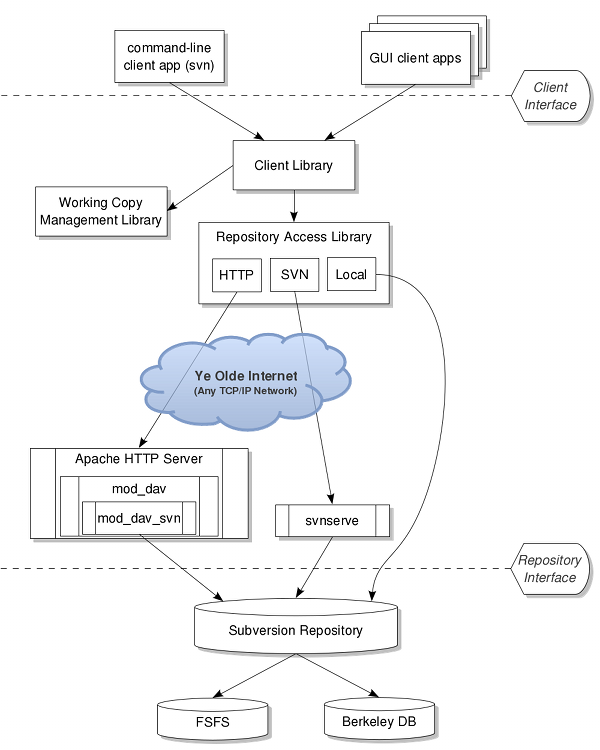
\includegraphics[width=5in,height=6.25in]{images/svn-arch-diagram.png}
\caption{Subversion\textquotesingle s
architecture}\label{svn.intro.architecture.dia-1}
\end{figure}

On one end is a Subversion repository that holds all of your versioned
data. On the other end is your Subversion client program, which manages
local reflections of portions of that versioned data. Between these
extremes are multiple routes through a Repository Access (RA) layer,
some of which go across computer networks and through network servers
which then access the repository, others of which bypass the network
altogether and access the repository directly.

\subsection{Subversion\textquotesingle s
Components}\label{svn.intro.components}

Subversion, once installed, has a number of different pieces. The
following is a quick overview of what you get. Don\textquotesingle t be
alarmed if the brief descriptions leave you scratching your
head---\emph{plenty} more pages in this book are devoted to alleviating
that confusion.

\begin{description}
\item[svn]
The command-line client program
\item[svnversion]
A program for reporting the state (in terms of revisions of the items
present) of a working copy
\item[svnlook]
A tool for directly inspecting a Subversion repository
\item[svnadmin]
A tool for creating, tweaking, or repairing a Subversion repository
\item[mod\_dav\_svn]
A plug-in module for the Apache HTTP Server, used to make your
repository available to others over a network
\item[svnserve]
A custom standalone server program, runnable as a daemon process or
invokable by SSH; another way to make your repository available to
others over a network
\item[svndumpfilter]
A program for filtering Subversion repository dump streams
\item[svnsync]
A program for incrementally mirroring one repository to another over a
network
\item[svnrdump]
A program for performing repository history dumps and loads over a
network
\item[svnmucc]
A program for performing multiple repository URL-based operations in a
single commit and without the use of a working copy
\end{description}

\subsection{What\textquotesingle s New in
Subversion}\label{svn.intro.whatsnew}

The first edition of this book was published by O\textquotesingle Reilly
Media in 2004, shortly after Subversion had reached 1.0. Since that
time, the Subversion project has continued to release new major releases
of the software. Here\textquotesingle s a quick summary of major new
changes since Subversion 1.0. Note that this is not a complete list; for
full details, please visit Subversion\textquotesingle s web site at
\href{https://subversion.apache.org}{}.

\begin{description}
\item[Subversion 1.1 (September 2004)]
Release 1.1 introduced FSFS, a flat-file repository storage option for
the repository. While the Berkeley DB backend is still widely used and
supported, FSFS has since become the default choice for newly created
repositories due to its low barrier to entry and minimal maintenance
requirements. Also in this release came the ability to put symbolic
links under version control, auto-escaping of URLs, and a localized user
interface.
\item[Subversion 1.2 (May 2005)]
Release 1.2 introduced the ability to create server-side locks on files,
thus serializing commit access to certain resources. While Subversion is
still a fundamentally concurrent version control system, certain types
of binary files (e.g. art assets) cannot be merged together. The locking
feature fulfills the need to version and protect such resources. With
locking also came a complete WebDAV auto-versioning implementation,
allowing Subversion repositories to be mounted as network folders.
Finally, Subversion 1.2 began using a new, faster binary-differencing
algorithm to compress and retrieve old versions of files.
\item[Subversion 1.3 (December 2005)]
Release 1.3 brought path-based authorization controls to the
\texttt{svnserve} server, matching a feature formerly found only in the
Apache server. The Apache server, however, gained some new logging
features of its own, and Subversion\textquotesingle s API bindings to
other languages also made great leaps forward.
\item[Subversion 1.4 (September 2006)]
Release 1.4 introduced a whole new tool---\texttt{svnsync}---for doing
one-way repository replication over a network. Major parts of the
working copy metadata were revamped to no longer use XML (resulting in
client-side speed gains), while the Berkeley DB repository backend
gained the ability to automatically recover itself after a server crash.
\item[Subversion 1.5 (June 2008)]
Release 1.5 took much longer to finish than prior releases, but the
headliner feature was gigantic: semi-automated tracking of branching and
merging. This was a huge boon for users, and pushed Subversion far
beyond the abilities of CVS and into the ranks of commercial competitors
such as Perforce and ClearCase. Subversion 1.5 also introduced a bevy of
other user-focused features, such as interactive resolution of file
conflicts, sparse checkouts, client-side management of changelists,
powerful new syntax for externals definitions, and SASL authentication
support for the \texttt{svnserve} server.
\item[Subversion 1.6 (March 2009)]
Release 1.6 continued to make branching and merging more robust by
introducing tree conflicts, and offered improvements to several other
existing features: more interactive conflict resolution options;
de-telescoping and outright exclusion support for sparse checkouts;
file-based externals definitions; and operational logging support for
\texttt{svnserve} similar to what \texttt{mod\_dav\_svn} offered. Also,
the command-line client introduced a new shortcut syntax for referring
to Subversion repository URLs.
\item[Subversion 1.7 (October 2011)]
Release 1.7 was primarily a delivery vehicle for two big plumbing
overhauls of existing Subversion components. The largest and most
impactful of these was the so-called ``WC-NG''---a complete rewrite of
the \texttt{libsvn\_wc} working copy management library. The second
change was the introduction of a sleeker HTTP protocol for Subversion
client/server interaction. Subversion 1.7 delivered a handful of
additional features, many bug fixes, and some notable performance
improvements, too.
\item[Subversion 1.8 (June 2013)]
In release 1.8, Subversion\textquotesingle s client now tracks renamed
files and directories more thoroughly, and its \texttt{svn\ merge}
command has grown intelligent enough to make the
\texttt{-\/-reintegrate} option unnecessary. Certain new versioned
property values can be inherited from parent directories. That feature
now allows a repository to dictate default values for automatic property
settings and ignorable file patterns, bringing consistency across the
user base of that repository in a way which previously had to be managed
socially. There is also a new built-in command-line file merge tool for
interactive conflict resolution. As always, Subversion 1.8 includes many
additional features, defect fixes, and improvements in behavior and
performance.
\end{description}

\section{Audience}\label{svn.preface.audience}

This book is written for computer-literate folk who want to use
Subversion to manage their data. While Subversion runs on a number of
different operating systems, its primary user interface is
command-line-based. That command-line tool (\texttt{svn}), and some
additional auxiliary programs, are the focus of this book.

For consistency, the examples in this book assume that the reader is
using a Unix-like operating system and is relatively comfortable with
Unix and command-line interfaces. That said, the \texttt{svn} program
also runs on non-Unix platforms such as Microsoft Windows. With a few
minor exceptions, such as the use of backward slashes
(\texttt{\textbackslash{}}) instead of forward slashes (\texttt{/}) for
path separators, the input to and output from this tool when run on
Windows are identical to those of its Unix counterpart.

Most readers are probably programmers or system administrators who need
to track changes to source code. This is the most common use for
Subversion, and therefore it is the scenario underlying all of the
book\textquotesingle s examples. But Subversion can be used to manage
changes to any sort of information---images, music, databases,
documentation, and so on. To Subversion, all data is just data.

While this book is written with the assumption that the reader has never
used a version control system, we\textquotesingle ve also tried to make
it easy for users of CVS (and other systems) to make a painless leap
into Subversion. Special sidebars may mention other version control
systems from time to time, and \hyperref[svn.forcvs]{Subversion for CVS
Users} summarizes many of the differences between CVS and Subversion.

Note also that the source code examples used throughout the book are
only examples. While they will compile with the proper compiler
incantations, they are intended to illustrate a particular scenario and
not necessarily to serve as examples of good programming style or
practices.

\section{How to Read This Book}\label{svn.preface.howread}

Technical books always face a certain dilemma: whether to cater to
``top-down'' or to ``bottom-up'' learners. A top-down learner prefers to
read or skim documentation, getting a large overview of how the system
works; only then does she actually start using the software. A bottom-up
learner is a ``learn by doing'' person---someone who just wants to dive
into the software and figure it out as she goes, referring to book
sections when necessary. Most books tend to be written for one type of
person or the other, and this book is undoubtedly biased toward top-down
learners. (And if you\textquotesingle re actually reading this section,
you\textquotesingle re probably already a top-down learner yourself!)
However, if you\textquotesingle re a bottom-up person,
don\textquotesingle t despair. While the book may be laid out as a broad
survey of Subversion topics, the content of each section tends to be
heavy with specific examples that you can try-by-doing. For the
impatient folks who just want to get going, you can jump right to
\hyperref[svn.intro]{Subversion Quick-Start Guide}.

Regardless of your learning style, this book aims to be useful to people
of widely different backgrounds---from those with no previous experience
in version control to experienced system administrators. Depending on
your own background, certain chapters may be more or less important to
you. The following can be considered a ``recommended reading list'' for
various types of readers:

\begin{description}
\item[Experienced system administrators]
The assumption here is that you\textquotesingle ve probably used version
control before and are dying to get a Subversion server up and running
ASAP. \hyperref[svn.reposadmin]{Repository Administration} and
\hyperref[svn.serverconfig]{Server Configuration} will show you how to
create your first repository and make it available over the network.
After that\textquotesingle s done, \hyperref[svn.tour]{Basic Usage} and
\hyperref[svn.forcvs]{Subversion for CVS Users} are the fastest routes
to learning the Subversion client.
\item[New users]
Your administrator has probably set up Subversion already, and you need
to learn how to use the client. If you\textquotesingle ve never used a
version control system, then \hyperref[svn.basic]{Fundamental Concepts}
is a vital introduction to the ideas behind version control.
\hyperref[svn.tour]{Basic Usage} is a guided tour of the Subversion
client.
\item[Advanced users]
Whether you\textquotesingle re a user or administrator, eventually your
project will grow larger. You\textquotesingle re going to want to learn
how to do more advanced things with Subversion, such as how to use
Subversion\textquotesingle s property support
(\hyperref[svn.advanced]{Advanced Topics}), how to use branches and
perform merges (\hyperref[svn.branchmerge]{Branching and Merging}), how
to configure runtime options (\hyperref[svn.customization]{Customizing
Your Subversion Experience}), and other things. These chapters
aren\textquotesingle t critical at first, but be sure to read them once
you\textquotesingle re comfortable with the basics.
\item[Developers]
Presumably, you\textquotesingle re already familiar with Subversion, and
now want to either extend it or build new software on top of its many
APIs. \hyperref[svn.developer]{Embedding Subversion} is just for you.
\end{description}

The book ends with reference material---\hyperref[svn.ref]{Subversion
Command Reference} is a reference guide for all Subversion commands, and
the appendixes cover a number of useful topics. These are the chapters
you\textquotesingle re most likely to come back to after
you\textquotesingle ve finished the book.

\section{Organization of This Book}\label{svn.preface.organization}

The chapters that follow and their contents are listed here:

\begin{description}
\item[{\hyperref[svn.basic]{Fundamental Concepts}}]
Explains the basics of version control and different versioning models,
along with Subversion\textquotesingle s repository, working copies, and
revisions.
\item[{\hyperref[svn.tour]{Basic Usage}}]
Walks you through a day in the life of a Subversion user. It
demonstrates how to use a Subversion client to obtain, modify, and
commit data.
\item[{\hyperref[svn.advanced]{Advanced Topics}}]
Covers more complex features that regular users will eventually come
into contact with, such as versioned metadata, file locking, and peg
revisions.
\item[{\hyperref[svn.branchmerge]{Branching and Merging}}]
Discusses branches, merges, and tagging, including best practices for
branching and merging, common use cases, how to undo changes, and how to
easily swing from one branch to the next.
\item[{\hyperref[svn.reposadmin]{Repository Administration}}]
Describes the basics of the Subversion repository, how to create,
configure, and maintain a repository, and the tools you can use to do
all of this.
\item[{\hyperref[svn.serverconfig]{Server Configuration}}]
Explains how to configure your Subversion server and offers different
ways to access your repository: \texttt{HTTP}, the \texttt{svn}
protocol, and local disk access. It also covers the details of
authentication, authorization and anonymous access.
\item[{\hyperref[svn.customization]{Customizing Your Subversion
Experience}}]
Explores the Subversion client configuration files, the handling of
internationalized text, and how to make external tools cooperate with
Subversion.
\item[{\hyperref[svn.developer]{Embedding Subversion}}]
Describes the internals of Subversion, the Subversion filesystem, and
the working copy administrative areas from a
programmer\textquotesingle s point of view. It also demonstrates how to
use the public APIs to write a program that uses Subversion.
\item[{\hyperref[svn.ref]{Subversion Command Reference}}]
Explains in great detail every subcommand of \texttt{svn},
\texttt{svnadmin}, and \texttt{svnlook} with plenty of examples for the
whole family!
\item[{\hyperref[svn.intro]{Subversion Quick-Start Guide}}]
For the impatient, a whirlwind explanation of how to install Subversion
and start using it immediately. You have been warned.
\item[{\hyperref[svn.forcvs]{Subversion for CVS Users}}]
Covers the similarities and differences between Subversion and CVS, with
numerous suggestions on how to break all the bad habits you picked up
from years of using CVS. Included are descriptions of Subversion
revision numbers, versioned directories, offline operations,
\texttt{update} versus \texttt{status}, branches, tags, metadata,
conflict resolution, and authentication.
\item[{\hyperref[svn.webdav]{WebDAV and Autoversioning}}]
Describes the details of WebDAV and DeltaV and how you can configure
your Subversion repository to be mounted read/write as a DAV share.
\item[{\hyperref[svn.copyright]{Copyright}}]
A copy of the Creative Commons Attribution License, under which this
book is licensed.
\end{description}

\section{This Book Is Free}\label{svn.preface.free}

This book started out as bits of documentation written by Subversion
project developers, which were then coalesced into a single work and
rewritten. As such, it has always been under a free license (see
\hyperref[svn.copyright]{Copyright}). In fact, the book was written in
the public eye, originally as part of the Subversion project itself.
This means two things:

\begin{itemize}
\item
  You will always find the latest version of this book in the
  book\textquotesingle s own Subversion repository.
\item
  You can make changes to this book and redistribute it however you
  wish---it\textquotesingle s under a free license. Your only obligation
  is to maintain proper attribution to the original authors. Of course,
  we\textquotesingle d much rather you send feedback and patches to the
  Subversion developer community, instead of distributing your private
  version of this book.
\end{itemize}

The online home of this book\textquotesingle s development and most of
the volunteer-driven translation efforts regarding it is
\href{https://svnbook.red-bean.com}{}. There you can find links to the
latest releases and tagged versions of the book in various formats, as
well as instructions for accessing the book\textquotesingle s Subversion
repository (where its DocBook XML source code lives). Feedback is
welcomed---encouraged, even. Please submit all comments, complaints, and
patches against the book sources to
\href{mailto:svnbook-dev@red-bean.com}{\nolinkurl{svnbook-dev@red-bean.com}}.

\section{Acknowledgments}\label{svn.preface.acks}

This book would not be possible (nor very useful) if Subversion did not
exist. For that, the authors would like to thank Brian Behlendorf and
CollabNet for the vision to fund such a risky and ambitious new open
source project; Jim Blandy for the original Subversion name and
design---we love you, Jim; and Karl Fogel for being such a good friend
and a great community leader, in that order.\footnote{Oh, and thanks,
  Karl, for being too overworked to write this book yourself.}

Thanks to O\textquotesingle Reilly and the team of professional editors
who have helped us polish this text at various stages of its evolution:
Chuck Toporek, Linda Mui, Tatiana Apandi, Mary Brady, and Mary Treseler.
Your patience and support has been tremendous.

Finally, we thank the countless people who contributed to this book with
informal reviews, suggestions, and patches. An exhaustive listing of
those folks\textquotesingle{} names would be impractical to print and
maintain here, but may their names live on forever in this
book\textquotesingle s version control history!

